\section{Extended Experimental Results}

%\vspace{10pt}
\subsection{Feature Similarity Analysis}
To further validate the effectiveness of the proposed GARD framework, we investigate the feature similarity across the transformer layers of the feed-forward reconstructor. Since the GARD denoiser is trained to map low-quality (LQ) degraded feature representations to their corresponding high-quality (HQ) clean representations, we measure the similarity between the restored representations and the clean representations to assess the extent to which the degraded feature representations are effectively recovered. Specifically, the feature similarity at transformer layer $l$ is computed as follows:
\begin{equation}
\mathrm{Sim}^{l} = 
\frac{
\mathbf{z}_{\text{res}}^{l}
\cdot 
\mathbf{z}_{\text{clean}}^{l}
}{
\left\lVert \mathbf{z}_{\text{res}}^{l} \right\rVert
\left\lVert \mathbf{z}_{\text{clean}}^{l} \right\rVert
},
\end{equation}
where $\mathbf{z}_{\text{res}}^{l}$ and $\mathbf{z}_{\text{clean}}^{l}$ are the restored and clean multi-view representations at layer $l$, respectively. Fig.~\ref{fig:suppl_feat_sim} visualizes this similarity for two independent scenes. In the baseline setting, without using the GARD denoiser, the similarity to the clean representation progressively decreases as the representations propagate through deeper layers, indicating that severe degradations cause a gradual loss of geometric information in the encoded features. In contrast, applying GARD at an early layer initially improves the similarity between restored and clean representations. These results provide a rationale for the improved reconstruction and pose estimation performance, demonstrating that GARD effectively maintains high-fidelity representations throughout the pipeline.
% \vspace{-5pt}
\begin{figure}[h]
    \centering
    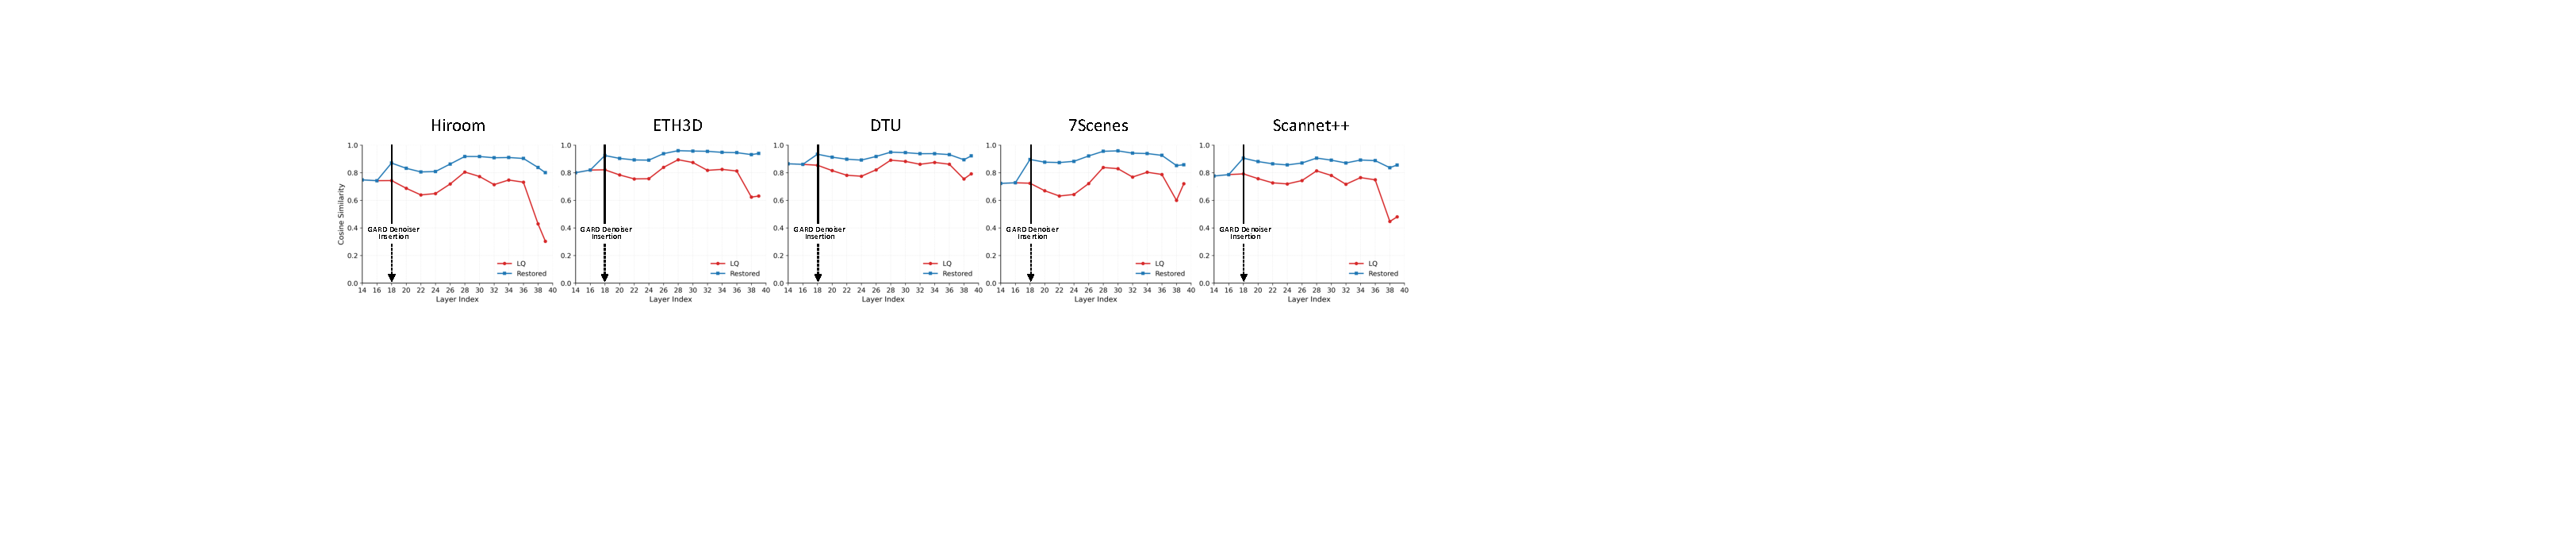
\includegraphics[width=\linewidth]{suppl/suppl_asset/JAE_camera_sim_figure_copy_2.pdf}
    \caption{
    \textbf{Feature similarity analysis across layers.}
    We evaluate the cosine similarity between the restored feature representations and the corresponding clean HQ representations across the multi-view encoder layers of the feed-forward 3D reconstruction model~\cite{depthanything3}. The GARD denoiser is applied at layer $K=18$. Across all DA3 benchmark~\cite{depthanything3} datasets, the feature similarity of the degraded LQ representations (red) progressively decreases in deeper layers due to the accumulation of degradation-induced feature distortion. In contrast, the restored representations produced by the GARD denoiser (blue) recover feature representations that remain substantially closer to the clean HQ representations throughout the deeper layers. This demonstrates that the GARD denoiser effectively restores geometry-aware features and suppresses degradation propagation, resulting in substantially improved consistency with the clean HQ representations. Please zoom in for clearer visualization.
    }
    \label{fig:suppl_feat_sim}
\end{figure}




\subsection{Feature Cost Volume Visualization}
Fig.~\ref{fig:suppl_cost_volume} further presents qualitative correspondence attention visualizations of the three feature cost volumes~\cite{kingma2013auto, oquab2023dinov2, depthanything3} analyzed in Fig.~\ref{fig:geo_aware} of the main paper. Specifically, for each red query point in the reference view, we visualize the attention region under (a) clean high-quality (HQ) multi-view inputs and (b) progressively increasing degradation levels of degraded multi-view inputs (mild, moderate, and heavy). Both quantitative and qualitative results reveal a clear performance hierarchy of DA3 $>$ DINOv2 $\gg$ VAE in terms of correspondence accuracy and robustness. Comparing the three feature cost volume representations through attention correspondence, DA3 features produce the sharpest and most geometrically consistent correspondences across views under both clean and degraded conditions, whereas DINOv2 achieves reasonably accurate matching with less precise and less stable response regions. In contrast, VAE features exhibit highly scattered and ambiguous correspondences under both clean and degraded conditions, reflecting limited geometry-aware representation quality caused by heavy latent compression. As the degradation severity increases, DA3 maintains strong localization and geometric consistency, whereas DINOv2 gradually deteriorates and VAE fails to preserve reliable correspondences.
\begin{figure}[h]
    \centering
    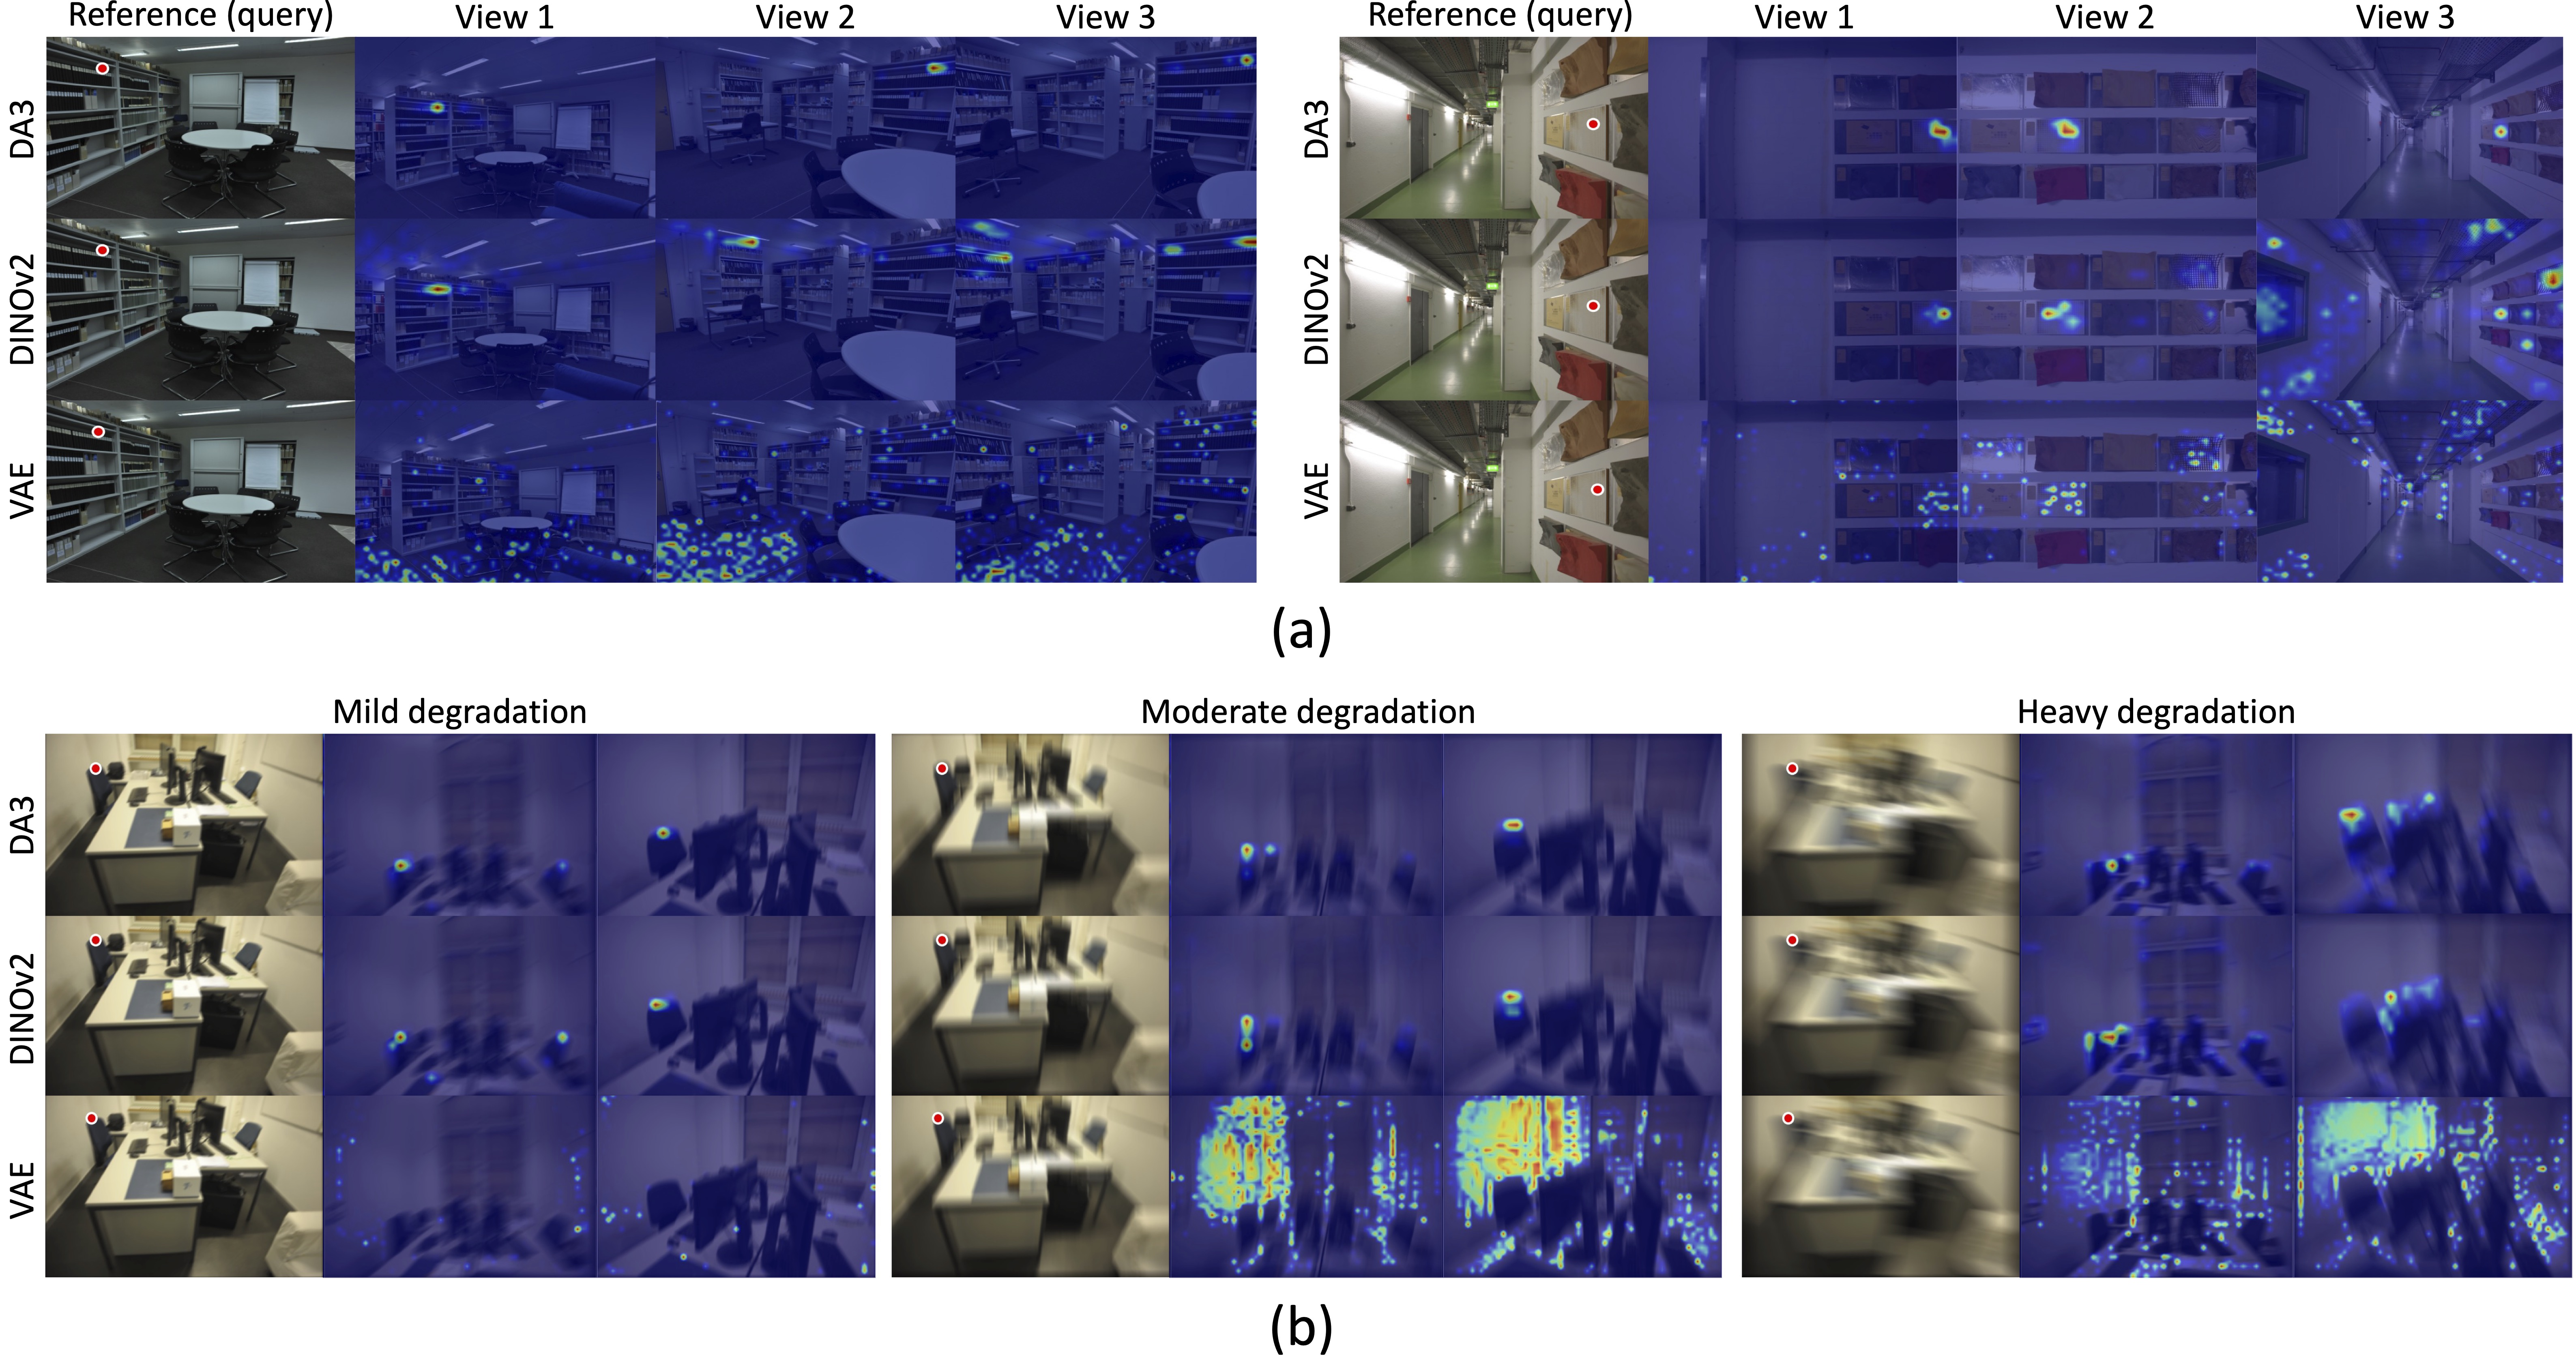
\includegraphics[width=0.95\linewidth]{suppl/suppl_asset/fig_geometry_aware_costvolume_copy_2.jpg}
    \caption{
    \textbf{Correspondence visualization of feature cost volumes.}
    Cross-view correspondence visualization of feature cost volumes constructed from VAE~\cite{kingma2013auto}, DINOv2~\cite{oquab2023dinov2}, and DA3~\cite{depthanything3} feature cost volumes. Please zoom in for clearer visualization.
    }
    \label{fig:suppl_cost_volume}
\end{figure}



\subsection{Multi-View Depth Estimation}
Tab.~\ref{supple_tab:da3_giant_depth} further presents the multi-view depth estimation evaluation. We report AbsRel$\downarrow$ and $\delta_1\uparrow$, which measure the absolute relative depth error and the percentage of predicted depths within a threshold ratio of $1.25$ from the ground-truth depth, respectively. GARD demonstrates superior depth estimation performance on the DA3~\cite{depthanything3} benchmark datasets, outperforming all baseline methods on four datasets while exhibiting only a marginal performance gap on DTU. These results underscore the effectiveness of restoration in a geometry-aware representation space for enhancing downstream multi-view depth estimation. By restoring degraded observations directly in this space, our method preserves cross-view geometric consistency and fine-grained structural details that are essential for accurate depth prediction. In contrast, single-view restoration methods are inherently unable to enforce geometric consistency across views, while VAE-based multi-view baselines are constrained by compression bottlenecks that limit the preservation of detailed geometric structures. As a result, baseline methods are more vulnerable to severe degradations, often producing blurred structures and visible artifacts, whereas our method yields sharper and more geometrically coherent depth maps across views, as further illustrated in the qualitative depth evaluation results in Fig.~\ref{fig:fig_suppl_depth}.
\begin{table*}[h]
\caption{\textbf{Quantitative depth estimation results.} We report AbsRel$\downarrow$ and $\delta_1\uparrow$ across the DA3 benchmarks~\cite{depthanything3}. The best result is highlighted in \textbf{bold} and the second best is \underline{underlined}.}
\label{supple_tab:da3_giant_depth}
\centering
%\setlength{\tabcolsep}{5pt}
%\renewcommand{\arraystretch}{1.1}

\resizebox{\linewidth}{!}{
\begin{tabular}{lccccc ccccc ccccc ccccc}
\toprule
\multirow{2}{*}{\textbf{Model}}
& \multicolumn{2}{c}{\textbf{HiRoom}}
& \multicolumn{2}{c}{\textbf{ETH3D}}
& \multicolumn{2}{c}{\textbf{DTU}}
& \multicolumn{2}{c}{\textbf{7Scenes}}
& \multicolumn{2}{c}{\textbf{ScanNet$++$}} \\
\cmidrule(lr){2-3} \cmidrule(lr){4-5} \cmidrule(lr){6-7} \cmidrule(lr){8-9} \cmidrule(lr){10-11}

& AbsRel$\downarrow$ & $\delta_1\uparrow$
& AbsRel$\downarrow$ & $\delta_1\uparrow$
& AbsRel$\downarrow$ & $\delta_1\uparrow$
& AbsRel$\downarrow$ & $\delta_1\uparrow$
& AbsRel$\downarrow$ & $\delta_1\uparrow$ \\
\midrule

\textit{Input Conditions} \\
\midrule
HQ Input
& 0.012 & 99.4
& 0.021 & 99.7
& 0.055 & 95.2
& 0.062 & 93.7
& 0.035 & 97.5 \\

LQ Input
& 0.191 & 78.6
& 0.087 & 90.4
& 0.061 & 94.5
& 0.137 & 81.9
& 0.092 & 89.5 \\

\midrule

\textit{Single-View Restoration} \\
\midrule

Restormer~\cite{zamir2022restormer}
& 0.210 & 74.1
& 0.140 & 82.2 
& 0.061 & 94.6
& 0.117 & 85.0
& 0.097 & 89.1 \\

HI-Diff~\cite{chen2023hierarchical}
& 0.239 & 70.2
& 0.105 & 86.3  
& 0.065 & 93.8
& 0.131 & 82.2
& 0.097 &  89.2 \\

InstructIR~\cite{conde2024high}
& 0.227 & 71.7
& 0.142 & 81.3 
& \underline{0.056} & 95.0
& 0.124 & 83.3
& 0.128 &  83.4 \\

MoCE-IR~\cite{zamfir2024complexityexperts}
& 0.198  &   76.8
& 0.096  &   88.3
& \textbf{0.055}  &   95.6
& 0.125  &   84.5
& 0.092  &   89.6
\\

\midrule

\textit{Multi-View Restoration} \\
\midrule

VRT~\cite{liang2024vrt}
& 0.193  &   77.9
& 0.087  &   90.2
& 0.060  &   94.7
& 0.144  &   80.5
& 0.092  &   89.8
\\

FMA-Net~\cite{Youk_2024_CVPR}
& 0.240 &    70.8
& 0.101 &    88.0
& 0.064 &    94.1
& 0.153 &    76.8
& 0.121 &    85.5
\\



VAE$_\text{MVD}$
& \underline{0.188} & \underline{80.2}
& \underline{0.069} & \underline{95.4}
& {0.057} & \underline{95.9}
& \underline{0.093} & \underline{89.0}
& \underline{0.068} & \underline{93.2} \\


\textbf{GARD (Ours)}
& \textbf{0.048} & \textbf{97.2}
& \textbf{0.036} & \textbf{98.4}
& {0.057} & \textbf{96.1}
& \textbf{0.071} & \textbf{92.7}
& \textbf{0.040} & \textbf{96.7}  \\

% \textbf{MVRM$_\text{GARDv2}$ (Ours)}
% &  &  
% &  &  
% &  &   
% &  &  
% &  &   \\

\bottomrule
\end{tabular}
}
\end{table*}





\subsection{Multi-View Restoration}
We additionally compare our method with SIR-Diff~\cite{mao2025sir}, a multi-view diffusion-based restoration model that leverages Spatial-3D ResNet blocks and 3D self-attention Transformers for effective restoration of degraded multi-view inputs. As the official pretrained checkpoints and training code were not publicly available, we contacted the authors for clarification and implemented the method based on the available unofficial training code together with the details provided in the paper. While we carefully followed the described training protocol to ensure a fair comparison, some components of the unofficial implementation were incomplete, which made full reproduction of the reported results challenging. Nevertheless, we made our best effort to faithfully follow the method as described. The quantitative comparisons are presented in Tab.~\ref{tab:sirdiff_compare}, and the qualitative results are provided in Fig.~\ref{fig:fig_suppl_sirdiff}. While SIR-Diff can produce reasonable restorations under mild degradation settings, its performance degrades noticeably under stronger corruption levels, where it often introduces artifacts and structural inconsistencies. As a result, its effectiveness for downstream geometric tasks becomes limited in challenging scenarios.
\vspace{-10pt}
\begin{table*}[h]
\centering
\subfloat[
\textbf{Pose estimation accuracy.} We report the area under the curve (AUC30)$\uparrow$ for pose evaluation.
\label{tab:sirdiff_pose}
]{
\begin{minipage}{0.48\linewidth}
\centering
\resizebox{\textwidth}{!}{
\begin{tabular}{lccccc}
\toprule
\multirow{2}{*}{\textbf{Model}} &
\multicolumn{5}{c}{AUC30$\uparrow$} \\
\cmidrule(lr){2-6}
& HiRoom & ETH3D & DTU & 7Scenes & ScanNet$++$ \\
\midrule
SIR-Diff~\cite{mao2025sir} & 9.73 & 20.94 & 16.59 & 2.79 & 30.02 \\
\textbf{GARD (Ours)} & \textbf{67.22} & \textbf{74.68} & \textbf{92.37} & \textbf{84.73} & \textbf{87.45} \\
\bottomrule
\end{tabular}}
\end{minipage}
}
\hfill
\subfloat[
\textbf{3D reconstruction accuracy.} We report Overall$\downarrow$ for DTU, while F-score$\uparrow$ is reported for the remaining benchmarks.
\label{tab:sirdiff_recon}
]{
\begin{minipage}{0.48\linewidth}
\centering
\resizebox{\textwidth}{!}{
\begin{tabular}{lccccc}
\toprule
\multirow{2}{*}{\textbf{Model}} &
\multicolumn{5}{c}{F-score$\uparrow$ / Overall$\downarrow$} \\
\cmidrule(lr){2-6}
& HiRoom & ETH3D & DTU & 7Scenes & ScanNet$++$ \\
\midrule
SIR-Diff~\cite{mao2025sir}  & 5.12 & 11.72 & 8.101 & 0.00 & 12.74 \\
\textbf{GARD (Ours)} & \textbf{18.25} & \textbf{45.79} & \textbf{4.760} & \textbf{36.08} & \textbf{35.77} \\
\bottomrule
\end{tabular}}
\end{minipage}
}
\vspace{-10pt}
\caption{\textbf{Quantitative evaluation of SIR-Diff~\cite{mao2025sir}.} We report the pose estimation and 3D reconstruction results on the DA3 benchmark~\cite{depthanything3}, comparing SIR-Diff~\cite{mao2025sir} with our GARD framework.}
\label{tab:sirdiff_compare}
% \vspace{-10pt}
\end{table*}




% \begin{table*}[t]
% \centering
% \subfloat[
% \textbf{Pose estimation accuracy.} We report the area under the curve (AUC@30)$\uparrow$ for camera pose evaluation under motion blur.
% \label{tab:sirdiff_compare_a}
% ]{
% \begin{minipage}{0.48\linewidth}
% \centering
% \resizebox{\textwidth}{!}{
% \begin{tabular}{lccccc}
% \toprule
% \textbf{Method} & HiRoom & ETH3D & DTU & 7Scenes & ScanNet$++$ \\
% \midrule
% SIRDiff~\cite{mao2025sir} & 9.74 & 20.9 & 16.6 & 2.79 & 30.0 \\
% \textbf{GARD (Ours)} & \textbf{67.2} & \textbf{74.7} & \textbf{92.4} & \textbf{84.7} & \textbf{87.4} \\
% \bottomrule
% \end{tabular}}
% \end{minipage}
% }
% \hfill
% \subfloat[
% \textbf{3D reconstruction accuracy.} We report Overall$\downarrow$ for DTU, while F-score$\uparrow$ is reported for the remaining benchmarks.
% \label{tab:sirdiff_compare_b}
% ]{
% \begin{minipage}{0.48\linewidth}
% \centering
% \resizebox{\textwidth}{!}{
% \begin{tabular}{lccccc}
% \toprule
% \textbf{Method} & HiRoom & ETH3D & DTU & 7Scenes & ScanNet$++$ \\
% \midrule
% SIRDiff~\cite{mao2025sir} & 5.12 & 11.72 & 1.67 & 0 & 12.74 \\
% \textbf{GARD (Ours)} & \textbf{18.26} & \textbf{45.79} & \textbf{4.760} & \textbf{36.09} & \textbf{35.78} \\
% \bottomrule
% \end{tabular}}
% \end{minipage}
% }
% \caption{\textbf{Comparison between VAE-based and geometry-aware multi-view restoration.} 
% We compare SIR-Diff~\cite{mao2025sir} and our GARD framework on pose estimation and 3D reconstruction under motion blur degradation.}
% \label{tab:sirdiff_compare}
% \vspace{-7pt}
% \end{table*}
\vspace{-15pt}
\begin{figure}[h]
    \centering
   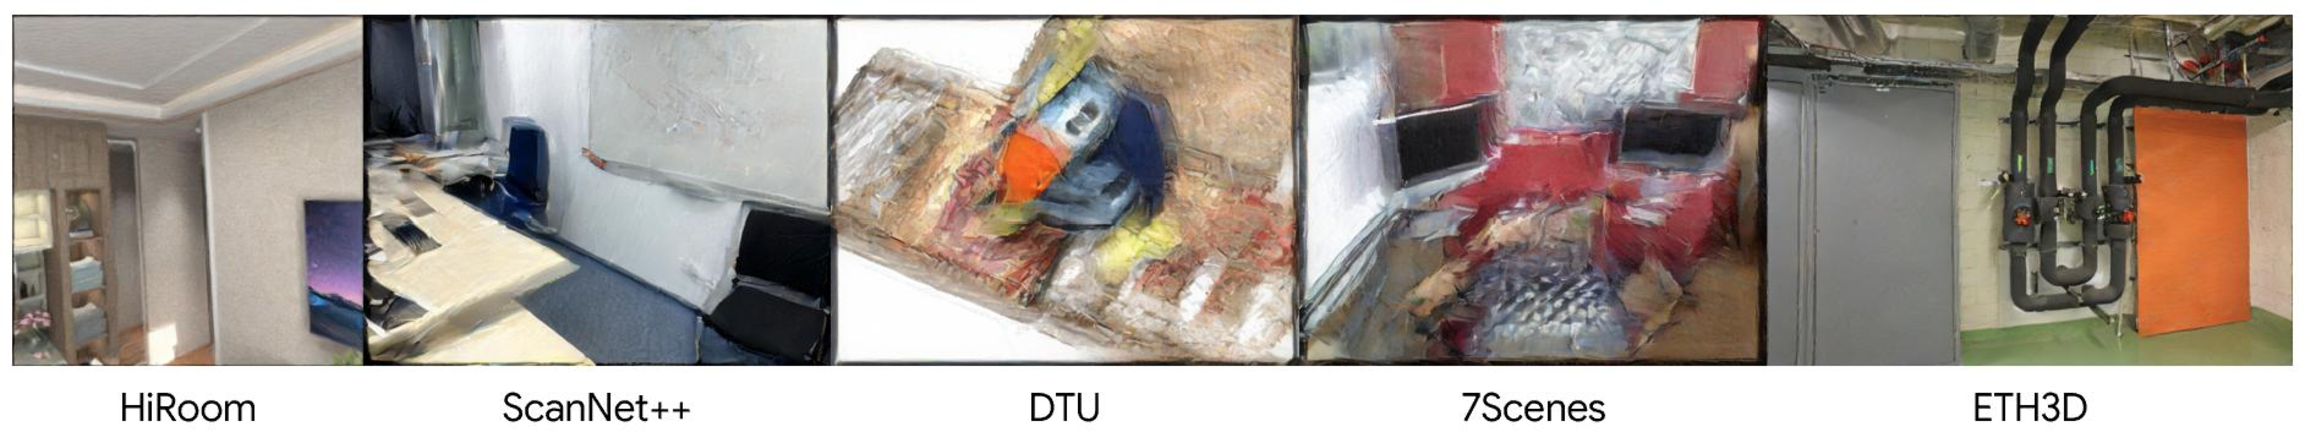
\includegraphics[width=0.95\linewidth]{suppl/suppl_asset/fig_suppl_sirdiff.pdf}
    \vspace{-5pt}
    \caption{\textbf{Multi-view image restoration results of SIR-Diff~\cite{mao2025sir}.} We show qualitative results on the DA3 benchmark~\cite{depthanything3} based on our reproduction of SIR-Diff.}
    \label{fig:fig_suppl_sirdiff}
\end{figure}



% As one of the representative multi-view restoration baselines, we carefully reproduced the SIR-Diff pipeline and evaluated the restored outputs using the same downstream geometric estimation framework. However, since the official implementation and pretrained checkpoints are not publicly available, exact reproduction was not possible. We further provide qualitative results of the reproduced SIR-Diff model in Fig.~\ref{fig:fig_suppl_3d_recon} under challenging degradation conditions. In our reproduction, the restored images generated by SIR-Diff still contained severe artifacts and structural distortions under strong degradations, which significantly degraded downstream geometric performance. Therefore, to ensure a fair comparison under the same evaluation setting, we additionally train and evaluate our GARD denoiser in the VAE-based latent space as a complementary baseline. Through this comparison, we demonstrate that denoising in a geometry-aware representation space is more effective for preserving cross-view consistency and accurate 3D geometry than restoration in a compressed VAE-based latent space.




\subsection{Multi-View Encoder Backbone}
We further evaluate the effectiveness of the GARD denoiser across encoder backbones of varying capacity by training it on a different multi-view encoder. Specifically, we train the GARD denoiser using representations from DA3-BASE. In contrast to DA3-GIANT, which comprises 40 transformer layers and 1.10B parameters, DA3-BASE consists of 12 layers and 0.11B parameters. Following the same design as DA3-GIANT, we apply the GARD denoiser within the DA3-BASE feature space by inserting it at encoder layer $K=4$, denoted as \textbf{GARD}$_{\textbf{BASE}}$. We report the pose estimation, 3D reconstruction, and depth estimation results in Tab.~\ref{tab:suppl_tab:da3_base_pose}, Tab.~\ref{supple_tab:da3_base_recon}, and Tab.~\ref{supple_tab:da3_base_depth}, respectively.
\begin{table*}[h]
\caption{\textbf{Quantitative pose estimation results.} We report AUC5$\uparrow$ and AUC30$\uparrow$ for camera pose estimation on the DA3 benchmark~\cite{depthanything3} using the DA3-BASE~\cite{depthanything3} checkpoint as the feed-forward 3D reconstruction model. The best result is highlighted in \textbf{bold} and the second best is \underline{underlined}.}
\label{tab:suppl_tab:da3_base_pose}
\centering
%\setlength{\tabcolsep}{4pt}
%\renewcommand{\arraystretch}{1.15}

\resizebox{\linewidth}{!}{
\begin{tabular}{lcccccccccccccccccccc}
\toprule
\multirow{2}{*}{\textbf{Model}}
& \multicolumn{2}{c}{\textbf{HiRoom}}
& \multicolumn{2}{c}{\textbf{ETH3D}}
& \multicolumn{2}{c}{\textbf{DTU}}
& \multicolumn{2}{c}{\textbf{7Scenes}}
& \multicolumn{2}{c}{\textbf{ScanNet$++$}} \\
\cmidrule(lr){2-3} \cmidrule(lr){4-5} \cmidrule(lr){6-7} \cmidrule(lr){8-9} \cmidrule(lr){10-11}

& AUC5$\uparrow$ & AUC30$\uparrow$
& AUC5$\uparrow$ & AUC30$\uparrow$
& AUC5$\uparrow$ & AUC30$\uparrow$
& AUC5$\uparrow$ & AUC30$\uparrow$
& AUC5$\uparrow$ & AUC30$\uparrow$ \\
\midrule

\textit{Input Conditions} \\
\midrule
% HQ Input
% & 35.14    & 84.05
% & 23.95    & 63.46
% & 53.13    & 91.05
% & 34.53    & 82.91
% & 37.62    & 69.70
% \\

HQ Input
&   35.21        &       84.11
&   23.79         &      62.61
&   53.53        &       91.21
&   34.47        &       83.02
&   37.68        &       69.81
\\

% LQ Input
% & \underline{0.53}    & 12.13
% & 1.01    & 11.30
% & 5.85    & 58.89
% & \underline{3.04}    & \underline{28.22}
% & \underline{4.37}    & \underline{33.29}
% \\

LQ Input
&   0.56    &   12.14   
&   1.01    &   11.44    
&   5.97    &   58.78    
&   3.04    &   28.26    
&   0.40    &   10.49
\\

\midrule

\textit{Single-View Restoration} \\
\midrule
% Restormer~\cite{zamir2022restormer}
% & 0.47    & \underline{12.85}
% & \underline{2.14}    & 17.33
% & 4.54    & 56.76
% & 0.00    & 2.70
% & 0.00    & 0.99    
% \\

Restormer~\cite{zamir2022restormer}
&   0.45    &       12.78
&   \underline{2.18}    &       17.25
&   4.44    &       56.56
&   4.88    &       48.20
&   \underline{5.20}    &       \underline{37.84}
\\


% HI-Diff~\cite{chen2023hierarchical}
% & 0.20    & 5.72
% & 1.17    &\underline{19.29}
% & 5.11    & 50.90
% & 0.00    & 2.15
% & 0.00    & 0.98
% \\

HI-Diff~\cite{chen2023hierarchical}
&   0.19    &       05.68
&   1.13    &       19.33
&   4.84    &       50.57
&   1.96    &       25.55
&   3.02    &       26.56
\\


% InstructIR~\cite{conde2024high}
% & 0.63   & 11.63
% & 1.37   & 16.34
% & \underline{22.72}  & \underline{75.97}
% & 0.00   & {3.52}
% & 0.00   & 1.48
% \\

InstructIR~\cite{conde2024high}
&   0.66    &       11.62
&   1.41    &       16.58
&   \underline{22.76}    &       \underline{76.01}
&   3.61    &        39.58
&   2.75    &       25.80
\\

MoCE-IR~\cite{zamfir2024complexityexperts}
&   0.91    &     17.15
&   2.02   &      \underline{22.36}
&   16.92    &     67.94  
&   4.12    &      35.75 
&   4.24    &     27.72   
\\


\midrule

\textit{Multi-View Restoration} \\
\midrule

VRT~\cite{liang2024vrt}
&    0.62   &    12.79   
&    1.65   &    16.70   
&    6.38   &    57.11   
&    1.33   &    24.21   
&    2.40   &    23.30
\\


FMA-Net~\cite{Youk_2024_CVPR}
&   0.04    &       06.92
&   0.80    &       15.35
&   2.52    &       36.87
&   0.25   &        12.96
&   1.00    &       19.15
\\


VAE$_\text{MVD}$
&    \underline{7.88}   &     \textbf{58.91  }
&    0.24   &     7.05 
&    11.11   &    60.42  
&    \underline{11.49}   &    \underline{51.48}
&    1.37   &     20.60
\\





% \textbf{GARD (Ours)}
% & \textbf{8.05}    & \textbf{58.60}
% & \textbf{6.58}    & \textbf{32.62}
% & \textbf{24.20}   & \textbf{76.14}
% & \textbf{4.01}    & \textbf{40.26}
% & \textbf{17.44}   & \textbf{56.13}
% \\

\textbf{GARD$_\textbf{BASE}$ (Ours)}
&    \textbf{8.14}   &       \underline{58.60}
&    \textbf{6.50}   &       \textbf{32.55}
&    \textbf{24.06}   &      \textbf{76.12}
&    \textbf{23.11}   &      \textbf{68.56}
&    \textbf{17.22}   &      \textbf{55.69}
\\




\bottomrule
\end{tabular}
}
\end{table*}




\begin{table*}[h]
\caption{\textbf{Quantitative 3D reconstruction results.} We report Overall$\downarrow$ and F-Score$\uparrow$ for 3D reconstruction on the DA3 benchmark~\cite{depthanything3} using the DA3-BASE~\cite{depthanything3} checkpoint as the feed-forward 3D reconstruction model. The best result is highlighted in \textbf{bold} and the second best is \underline{underlined}.}
\label{supple_tab:da3_base_recon}
\centering

\resizebox{\linewidth}{!}{
\begin{tabular}{lccccccccc}
\toprule
\multirow{2}{*}{\textbf{Model}}
& \multicolumn{2}{c}{\textbf{HiRoom}}
& \multicolumn{2}{c}{\textbf{ETH3D}}
& \multicolumn{1}{c}{\textbf{DTU}}
& \multicolumn{2}{c}{\textbf{7Scenes}}
& \multicolumn{2}{c}{\textbf{ScanNet$++$}} \\
\cmidrule(lr){2-3}
\cmidrule(lr){4-5}
\cmidrule(lr){6-6}
\cmidrule(lr){7-8}
\cmidrule(lr){9-10}

& Overall$\downarrow$ & F-score$\uparrow$
& Overall$\downarrow$ & F-score$\uparrow$
& Overall$\downarrow$
& Overall$\downarrow$ & F-score$\uparrow$
& Overall$\downarrow$ & F-score$\uparrow$ \\
\midrule

\multicolumn{10}{l}{\textit{Input Conditions}} \\
\midrule

% HQ Input
% & 0.349 & 22.2
% & 1.229 & 37.1
% & 5.811
% & 0.187 & 32.0
% & 0.340 & 26.1 
% \\

HQ Input
&  0.349     &      22.29
&  1.220     &      37.92
&  5.843
&  0.186     &      31.89
&  0.340    &       26.09
\\

% LQ Input
% & \underline{0.931} & 7.5
% & 3.455 & 11.8
% & 8.417
% & \underline{0.529} & \underline{12.6}
% & \underline{0.474} & \underline{13.1} 
% \\

LQ Input
&  0.946     &      7.58
&  3.337     &      11.85
&  8.429
&  0.529     &      12.56
&  \underline{0.476}    &       \underline{13.12}
\\


\midrule


\multicolumn{10}{l}{\textit{Single-View Restoration}} \\
\midrule

% Restormer~\cite{zamir2022restormer}
% & 1.124 & \underline{7.60}
% & \underline{3.084} & \underline{14.5}
% & 9.106
% & 1.599 & 0.00
% & 1.370 & 1.83 
% \\

Restormer~\cite{zamir2022restormer}
&   0.889    &       7.67
&   3.212    &       \underline{14.67}
&   9.064
&   0.755   &       13.24
&   0.489   &       12.16
\\


% HI-Diff~\cite{chen2023hierarchical}
% & 1.605 & 4.52
% & 3.753 & 8.01
% & 8.847
% & 1.617 & 0.00
% & 1.217 & 2.12 
% \\

HI-Diff~\cite{chen2023hierarchical}
&   1.173    &       4.58
&   3.737     &      8.02
&   8.826
&   0.551   &       12.95
&   0.612    &      8.33
\\

% InstructIR~\cite{conde2024high}
% & 1.027 & 6.12
% & 3.560 & 8.05
% & \underline{7.972}
% & 1.601 & 0.00
% & 1.327 & 1.83 
% \\

InstructIR~\cite{conde2024high}
&  1.183     &     6.23
&  3.653    &      7.29
&  7.960
&  0.501     &     14.19
&  0.562    &      9.03
\\

MoCE-IR~\cite{zamfir2024complexityexperts}
&   0.870   &      7.81
&   \underline{2.909}    &     13.95
&   7.942   
&   0.504    &     12.17
&   0.554   &      9.45 
\\


\midrule

\multicolumn{10}{l}{\textit{Multi-View Restoration}} \\
\midrule

VRT~\cite{liang2024vrt}
&    0.882   &     7.87  
&    3.226   &     10.68 
&    8.770  
&    0.750   &     6.98
&    0.558   &     8.96  
\\


FMA-Net~\cite{Youk_2024_CVPR}
&   1.319    &   4.45
&   3.623    &   11.92
&   8.653    
&   1.171    &   4.53
&   0.813    &   5.80
\\


VAE$_\text{MVD}$
&   \textbf{0.389}    &     \underline{11.63}
&   5.518    &     4.63
&   \underline{7.571}
&   \underline{0.314}    &    \underline{20.15}
&   0.636    &    6.21
\\


% \textbf{GARD (Ours)}
% & \textbf{0.513}    & \textbf{12.72}
% & \textbf{1.996}    & \textbf{20.71}
% & \textbf{6.323} 
% & \textbf{0.498}    & \textbf{14.25}
% & \textbf{0.347}    & \textbf{21.52}
% \\

\textbf{GARD$_\text{BASE}$ (Ours)}
&  \underline{0.512}    &    \textbf{12.69}
&  \textbf{2.047}   &     \textbf{20.38}  
&  \textbf{6.304}
&  \textbf{0.232}     &     \textbf{23.41}
&  \textbf{0.347}     &     \textbf{21.60}  
\\


\bottomrule
\end{tabular}
}

\end{table*}
\begin{table*}[h]
\caption{\textbf{Quantitative depth estimation results.} We report AbsRel$\downarrow$ and $\delta_1\uparrow$ on the DA3 benchmark~\cite{depthanything3} using the DA3-BASE~\cite{depthanything3} checkpoint as the feed-forward 3D reconstruction model. The best result is highlighted in \textbf{bold} and the second best is \underline{underlined}.}
\label{supple_tab:da3_base_depth}
\centering
%\setlength{\tabcolsep}{5pt}
%\renewcommand{\arraystretch}{1.1}

\resizebox{\linewidth}{!}{
\begin{tabular}{lccccc ccccc ccccc ccccc}
\toprule
\multirow{2}{*}{\textbf{Model}}
& \multicolumn{2}{c}{\textbf{HiRoom}}
& \multicolumn{2}{c}{\textbf{ETH3D}}
& \multicolumn{2}{c}{\textbf{DTU}}
& \multicolumn{2}{c}{\textbf{7Scenes}}
& \multicolumn{2}{c}{\textbf{ScanNet$++$}} \\
\cmidrule(lr){2-3} \cmidrule(lr){4-5} \cmidrule(lr){6-7} \cmidrule(lr){8-9} \cmidrule(lr){10-11}

& AbsRel$\downarrow$ & $\delta_1\uparrow$
& AbsRel$\downarrow$ & $\delta_1\uparrow$
& AbsRel$\downarrow$ & $\delta_1\uparrow$
& AbsRel$\downarrow$ & $\delta_1\uparrow$
& AbsRel$\downarrow$ & $\delta_1\uparrow$ \\
\midrule

\textit{Input Conditions} \\
\midrule
% HQ Input
% & 0.012 & 99.4
% & 0.021 & 99.70
% & 0.055 & 95.2
% & 0.062 & 93.7
% & 0.035 & 97.5 
% \\

HQ Input
&    0.039   &       98.28
&    0.035   &      98.89
&    0.051   &      97.13
&    0.068  &       93.50
&    0.044   &       97.08
\\


% LQ Input
% & 0.191 & 78.6
% & 0.087 & 90.4
% & 0.061 & 94.5
% & 0.137 & 81.9
% & 0.092 & 89.5 
% \\

LQ Input
&   0.195    &       77.75
&   0.124    &      84.75
&   0.057   &       95.66
&   0.144    &      79.19
&   0.123    &      85.07
\\



\midrule

\textit{Single-View Restoration} \\
\midrule

% Restormer~\cite{zamir2022restormer}
% & 0.21 & 74.1
% & 0.14 & 82.2 
% & 0.061 & 94.6
% & 0.117 & 85.0
% & 0.097 & 89.1 
% \\

Restormer~\cite{zamir2022restormer}
&   0.202    &      76.56
&   0.147    &      80.91
&   0.057    &       95.71
&   0.119    &      84.47
&   \underline{0.112}    &      \underline{86.36}
\\


% HI-Diff~\cite{chen2023hierarchical}
% & 0.2389 & 70.2
% & 0.105 & 86.3  
% & 0.065 & 93.8
% & 0.131 & 82.2
% & 0.097 &  89.2 
% \\

HI-Diff~\cite{chen2023hierarchical}
&   0.237    &       71.45
&   0.122    &       84.88
&   0.063    &       94.36
&   0.143    &       80.08
&   0.131    &       84.02
\\

% InstructIR~\cite{conde2024high}
% & 0.227 & 71.7
% & 0.142 & 81.3 
% & \textbf{0.056} & 95.0
% & 0.124 & 83.3
% & 0.128 &  83.4 
% \\

InstructIR~\cite{conde2024high}
&   0.215    &       74.66
&   0.142    &       81.43
&   \underline{0.054}   &      \underline{95.94}
&   0.123    &       83.69
&   0.143    &       82.27
\\


MoCE-IR~\cite{zamfir2024complexityexperts}
&  0.186     &       79.12
&  0.124     &       85.07
&  \textbf{0.053}     &       \textbf{96.16}
&  0.132     &       81.52
&  0.122    &        85.51
\\


\midrule
\textit{Multi-View Restoration} \\
\midrule

VRT~\cite{liang2024vrt}
&   0.195    &      77.72
&   \underline{0.122}    &      \underline{85.24}
&   0.056    &      95.93
&   0.147    &      78.14
&   0.125    &      84.70
\\


FMA-Net~\cite{Youk_2024_CVPR}
&   0.251    &       69.54
&   0.137    &       82.12
&   0.063    &       95.13
&   0.178    &       73.26
&   0.159    &       79.07
\\


VAE$_\text{MVD}$
&    \underline{0.099}   &       \underline{92.80}
&    0.248   &       63.74
&    \underline{0.054}   &       95.85
&    \underline{0.106}   &       \underline{87.43}
&    0.160   &        77.57
\\



% \textbf{GARD (Ours)}
% & \textbf{0.201} & \textbf{97.2}
% & \textbf{0.036} & \textbf{98.4}
% & \underline{0.057} & \textbf{95.1}
% & \textbf{0.0707} & \textbf{92.7}
% & \textbf{0.040} & \textbf{96.7}  
% \\

\textbf{GARD$_\text{BASE}$ (Ours)}
&   \textbf{0.079}    &   \textbf{95.04}
&   \textbf{0.063}    &   \textbf{95.54}
&   0.060    &   95.23
&   \textbf{0.081}   &    \textbf{91.60}
&   \textbf{0.059}    &   \textbf{95.76}
\\


\bottomrule
\end{tabular}
}
\end{table*}


